%settings

\setlength{\parindent}{2ex}
\phantomsection
%text
%-Task1----------------------------------
\section{Model of the project with Class Diagrams.}
\begin{figure}[h!]
	\centering
	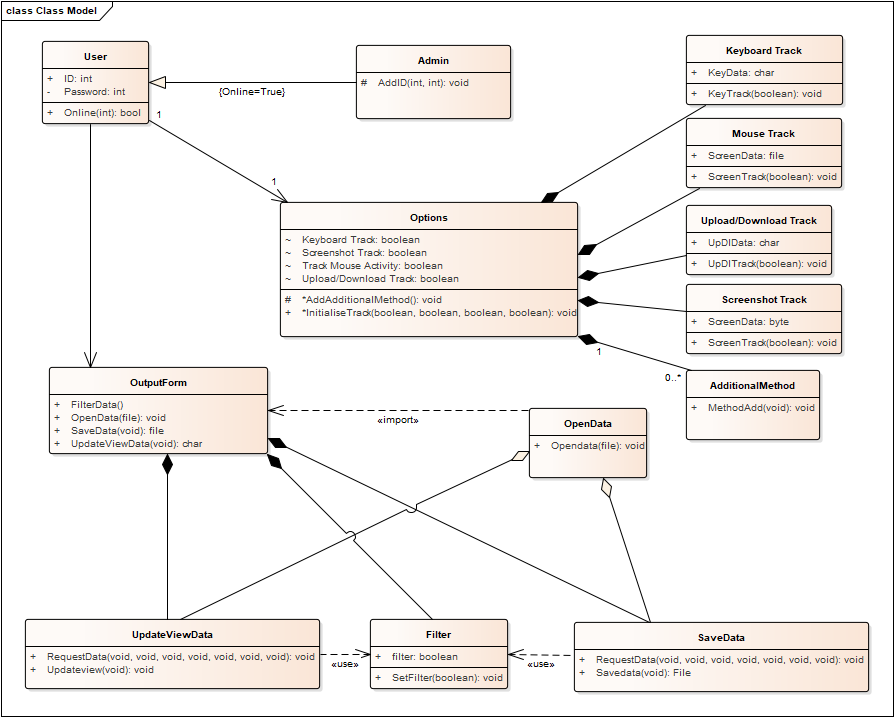
\includegraphics[width=\textwidth]{ClassModel}
	\caption{Class Diagram} 
\end{figure}
The class diagram in \textbf{Figure \thesection.1} contains the general conceptual modeling of the application classes used.
\par
The most important classes in this project are:
\begin{itemize}
\item[•] User class.\textit{(Class that responds for the user functionality)}
\item[•] Options class.\textit{(Class that responds for the option selection and tracking methods instantiation)}
\item[•] OutputForm class.\textit{(Class that responds for the tracked data operations)}
\end{itemize}
The User can be further generalized in Admin class that overwrites the User variables and has the ability to add other Users Id's to track.
\par
Each user is associated with a option selection class and through it the user selects the tracking methods and then after the selection track methods are initialized; if the user choose an additional method then .
\par
The OutputForm is the class that deals with data manipulation and its representation.
\begin{itemize}
\item Open data responds for opening the files that contain tracked data and use the other other functions of generalized class OutputForm. 
\item UpdateViewsData outputs on interface on screen that is processed and requested from the track methods and filter.
\item Filter filters the data according to the user input.
\item Save data saves the data that is processed and requested from the track methods and filter.
\end{itemize}



%-Task2----------------------------------
%\newpage
\section{SWOT analysis of the project.}
The SWOT analysis of the project is explained below in the Figure \thesection.1 .
\begin{figure}[h!]
	\centering
	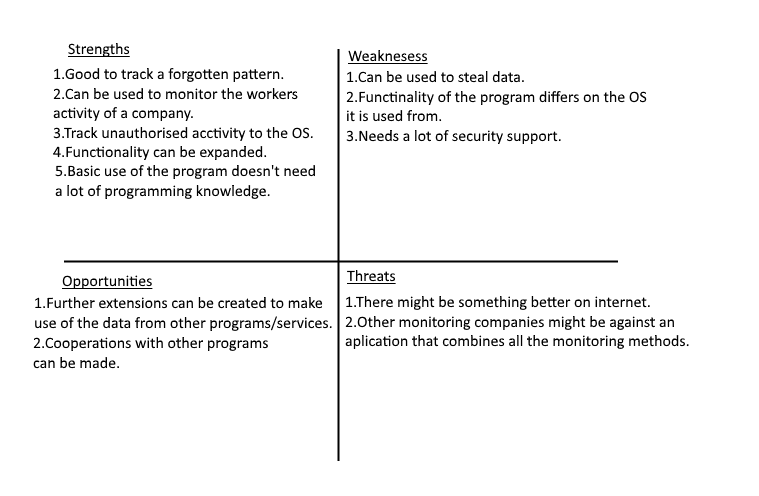
\includegraphics[width=\textwidth]{SWOT}
	\caption{SWOT} 
\end{figure}
\clearpage
